% Panels for causal-knowledge-graphs.tex. The manuscript is twocolumn,
% so every panel is a figure* spanning both columns.
% Generated by figures/generate_panels.py -- every plotted number is
% recomputed at draw time from the coordinates of Table~\ref{tab:aa}.

\begin{figure*}[!htbp]
\centering
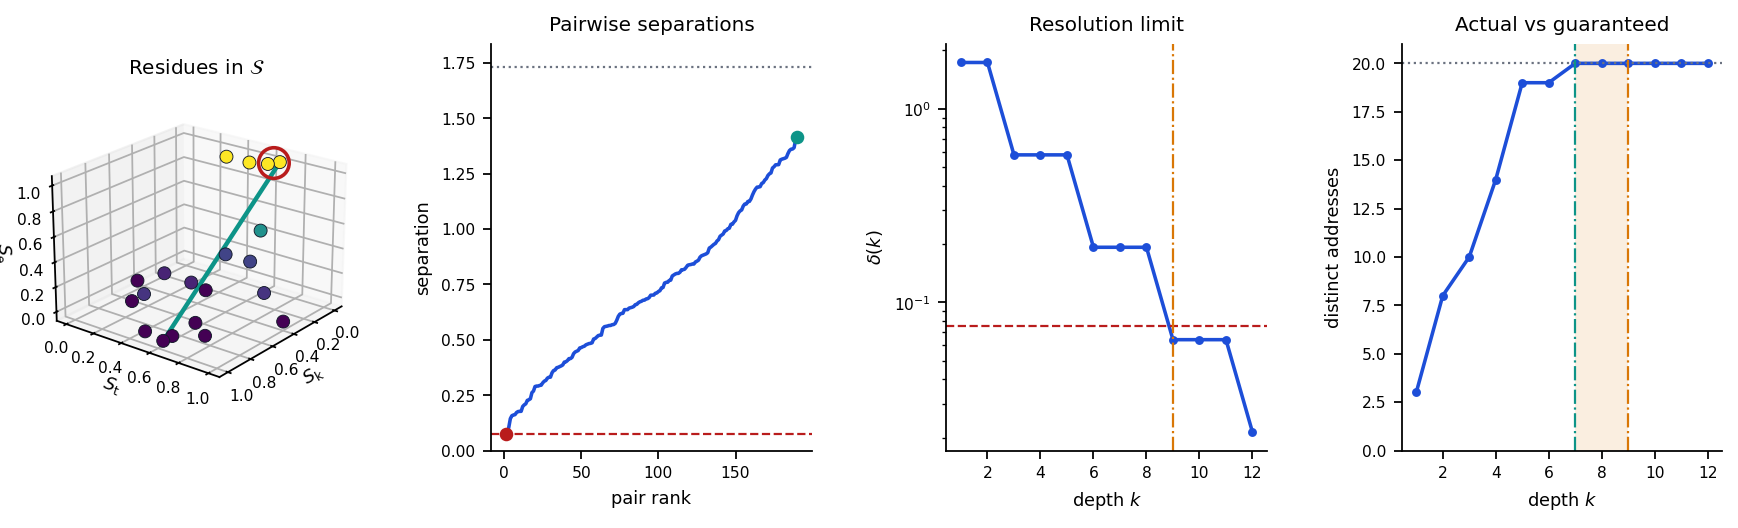
\includegraphics[width=\textwidth]{figures/panel_01_encoding.png}
\caption{\textbf{S-entropy coordinates and the resolution they force.}
(\textbf{A})~The twenty canonical residues in the S-entropy cube
$\Sspace = [0,1]^3$, coloured by $S_{\mathrm{e}}$. The teal segment is the
farthest realised pair, Ile--Arg at $d_{\max} = 1.415$; the red ring marks
Lys--Arg, the closest pair at $d_{\min} = 0.0756$, which is sub-pixel at
this scale and so is ringed rather than drawn.
(\textbf{B})~All $190$ pairwise separations in increasing order. The lower
dashed line is $d_{\min}$, the upper dotted line the cube diameter
$\sqrt3$; the curve terminates well short of it.
(\textbf{C})~The cell diagonal $\delta(k) = \sqrt3\,3^{-\lfloor k/3\rfloor}$
against $d_{\min}$. The two first meet at $k=9$, which is therefore the
guaranteed resolution depth of \Cref{thm:aa-resolution}, and the guarantee
is tight: $\delta(8) = 0.1925 > d_{\min}$.
(\textbf{D})~Addresses that are actually distinct at each depth. All twenty
separate at $k=7$ (teal), two levels below the $k=9$ guarantee (orange);
the shaded band is the slack recorded in \Cref{rem:guarantee-slack}.}
\label{fig:panel-encoding}
\end{figure*}

\begin{figure*}[!htbp]
\centering
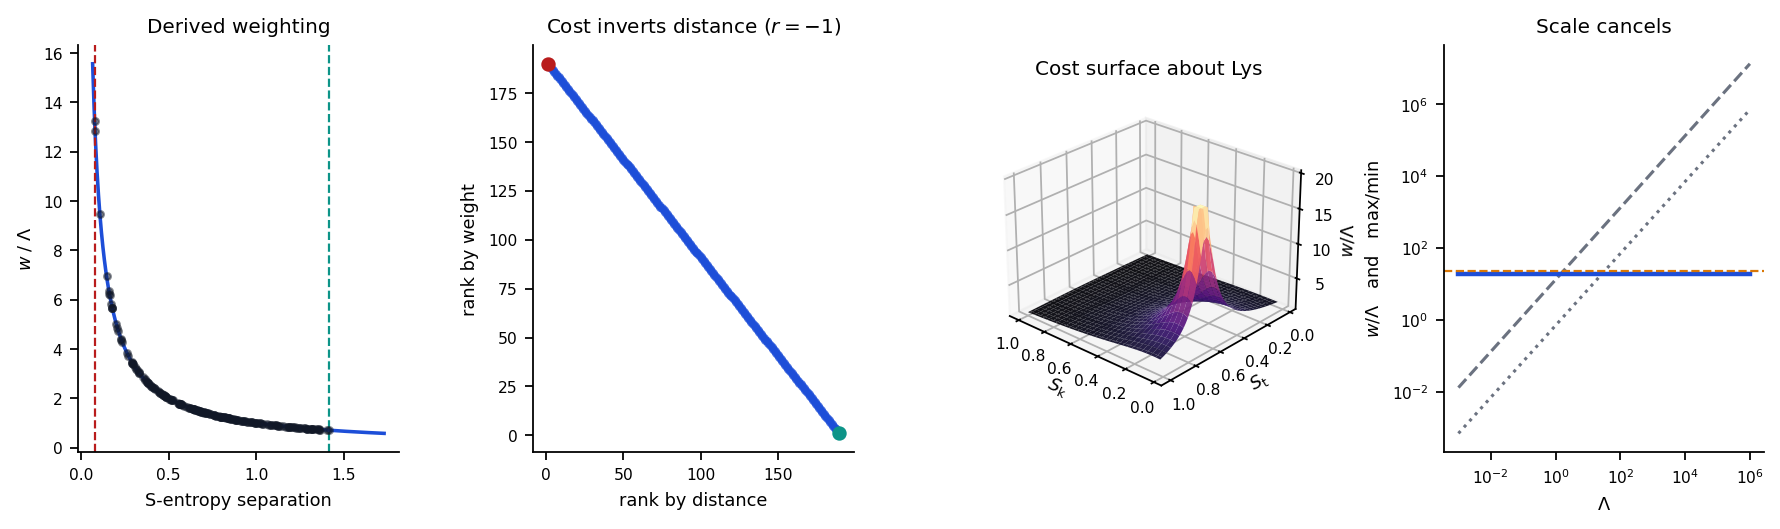
\includegraphics[width=\textwidth]{figures/panel_02_weighting.png}
\caption{\textbf{The derived contact weighting is a separation cost.}
(\textbf{A})~The weighting $\wt = \Lambda/\norm{\sse(u)-\sse(v)}$ of
\eqref{eq:wt-derived}, with the $190$ residue pairs overlaid. Dashed lines
mark $d_{\min}$ and $d_{\max}$.
(\textbf{B})~Each pair ranked independently by S-entropy distance and by
contact weight, both ascending. The rankings are exactly reversed
($r = -1$): the closest pair (red) is the most expensive to separate and
the farthest (teal) the cheapest, which is the inversion of
\Cref{rem:reciprocal} and the sense in which $\wt$ measures cost rather
than distance.
(\textbf{C})~The cost surface over an $(S_{\mathrm{k}}, S_{\mathrm{t}})$
slice through Lys, clipped at $20\Lambda$. Contact strength is a pole at
the reference residue, not a bounded similarity score.
(\textbf{D})~Individual weights (grey) sweep nine decades as $\Lambda$
varies, while their ratio (blue) does not move. The scale cancels from
every prediction, so the theory carries no fitted parameter; the orange
line is the bound $\sqrt3/d_{\min}$.}
\label{fig:panel-weighting}
\end{figure*}

\begin{figure*}[!htbp]
\centering
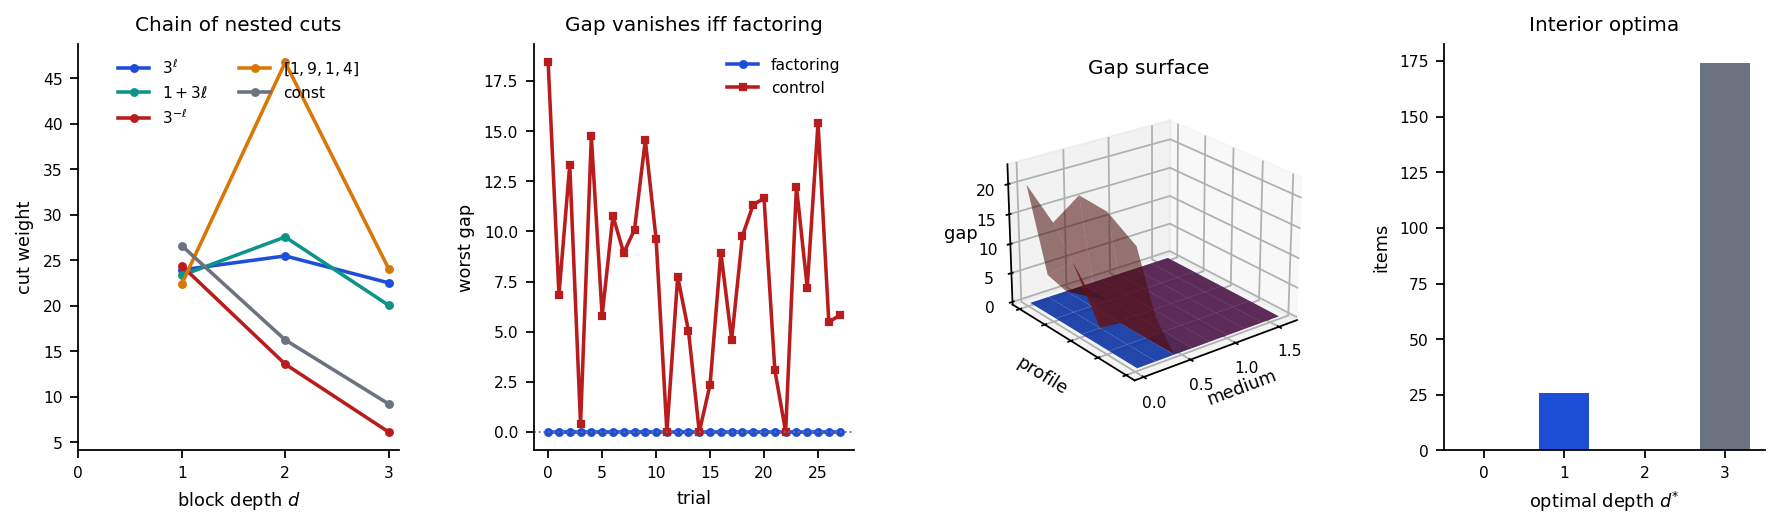
\includegraphics[width=\textwidth]{figures/panel_03_subtrie_cut.png}
\caption{\textbf{Minimum cuts land on trie boundaries, and only under the
factoring hypothesis.}
(\textbf{A})~Cut weight along the chain of nested subtrie blocks
$B_d(v)$ for five weight profiles: increasing, linear, decreasing,
non-monotone and constant. Depth $d=0$ is the degenerate whole-set cut and
is excluded throughout (\Cref{rem:degenerate-cuts}). That decreasing and
non-monotone profiles behave no differently is
\Cref{rem:factoring-not-monotone} made visible.
(\textbf{B})~The gap \eqref{eq:gap} between the chain minimum and the true
minimum over all $2^{\abs{\V}-1}$ admissible cuts. Under factoring (blue)
it is identically zero; under weights drawn independently per pair (red),
with every other feature of the instance preserved, it reaches $18.4$.
(\textbf{C})~The same contrast as a surface over medium coupling and weight
profile: the factoring sheet (blue) is flat at zero everywhere, the control
sheet (red) is not.
(\textbf{D})~Where the optimum sits. Grey bars are the two degenerate
depths, $d^{*}=0$ and $d^{*}=k$; the blue bar counts items whose optimal
block is strictly interior, confirming the result is not an artefact of the
trivial minimisers.}
\label{fig:panel-subtrie}
\end{figure*}

\begin{figure*}[!htbp]
\centering
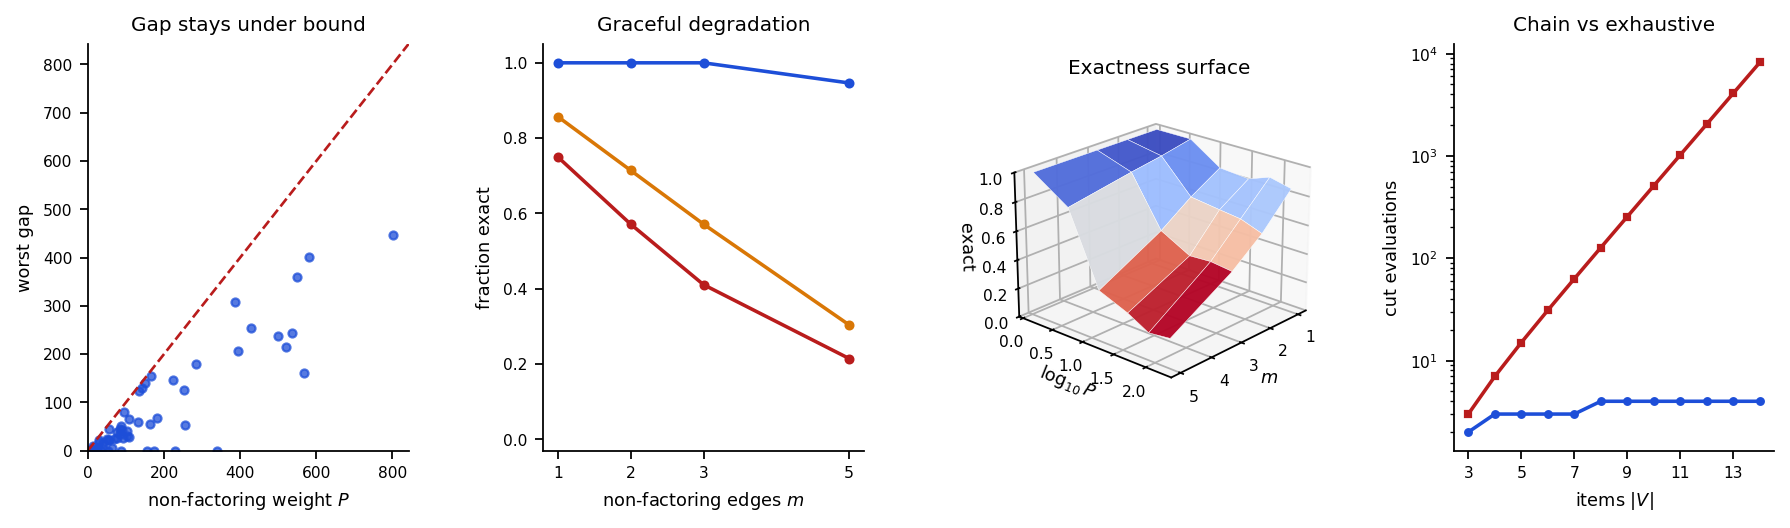
\includegraphics[width=\textwidth]{figures/panel_04_degradation.png}
\caption{\textbf{Degradation when the factoring hypothesis fails.}
Real contact graphs carry disulfides and other couplings that violate
\eqref{eq:trie-factoring}; these charts perturb a factoring graph by adding
$m$ such edges of total weight $P$.
(\textbf{A})~The gap against $P$ over all trials. Every point lies below the
identity (dashed), so the bound of \Cref{rem:complexity-honest} holds, and
points approach it closely enough ($\gapv/P$ up to $0.938$) that it is not
slack.
(\textbf{B})~Fraction of items whose separation cost is still computed
exactly, against the number of offending edges, at three perturbation
magnitudes. Degradation is monotone rather than catastrophic.
(\textbf{C})~The same quantity as a surface over $m$ and $\log_{10}P$.
Exactness falls monotonically in both directions, from unity under weak
single couplings to below $0.3$ under many strong ones.
(\textbf{D})~Cut evaluations required: $k+1$ along the chain against
$2^{\abs{\V}-1}$ exhaustively, on a logarithmic axis. This is the content
of \Cref{cor:sepcost-cheap}, counted directly rather than quoted
asymptotically.}
\label{fig:panel-degradation}
\end{figure*}

\begin{figure*}[!htbp]
\centering
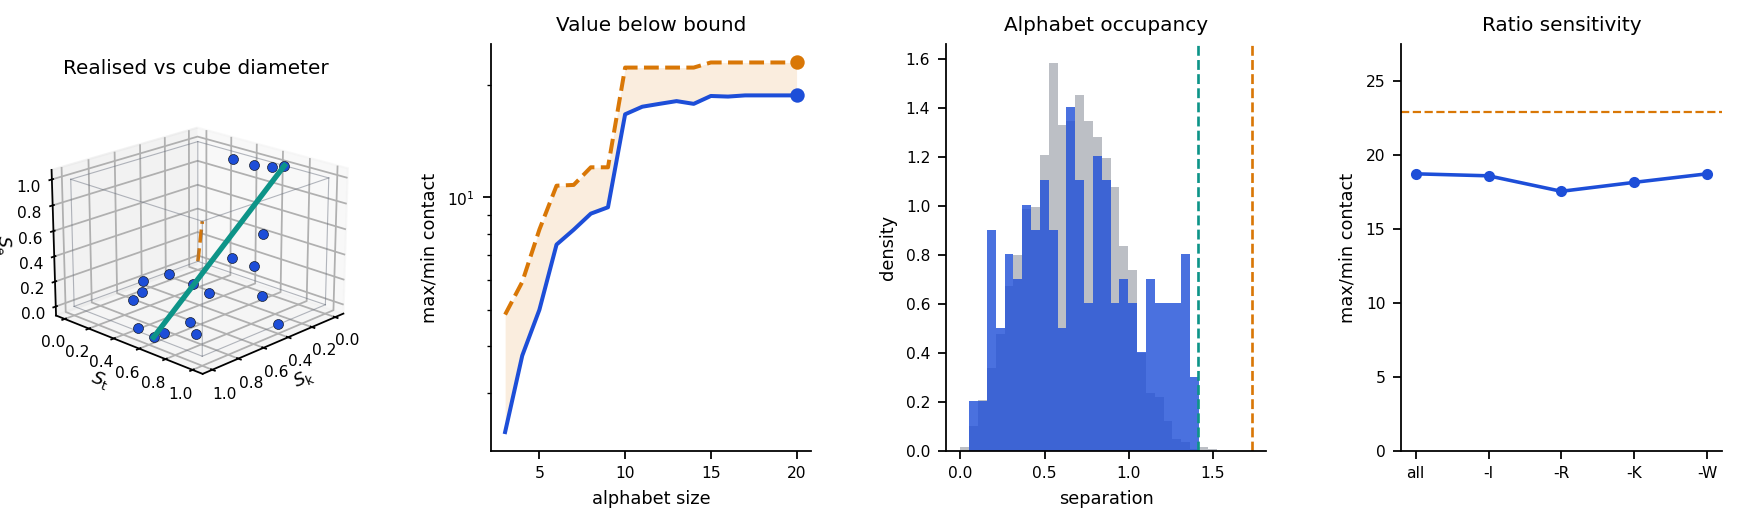
\includegraphics[width=\textwidth]{figures/panel_05_ratio.png}
\caption{\textbf{A bound distinguished from a value.}
(\textbf{A})~The residues in $\Sspace$ with the unit cube drawn. The teal
segment is the farthest realised pair, Ile--Arg; the orange dashed line is
the cube diagonal. They are not the same object, which is the whole content
of \Cref{rem:ratio-bound}: $\sqrt3$ is the diameter of the cube, and no two
residues occupy opposite corners.
(\textbf{B})~The realised contact ratio $d_{\max}/d_{\min}$ (blue) against
the bound $\sqrt3/d_{\min}$ (orange) for random sub-alphabets of increasing
size. The shaded band between them is the overstatement the validation
caught; it narrows as the alphabet fills the cube, closing at $18.7$
against $22.9$ for the full twenty.
(\textbf{C})~Distribution of residue separations (blue) against separations
between uniformly random points of the cube (grey). The alphabet reaches
$82\%$ of the available diameter --- spread through $\Sspace$, but not to
its extremes (\Cref{rem:alphabet-occupancy}).
(\textbf{D})~Sensitivity of the ratio to removing each residue of the
extreme pairs. It moves by less than $7\%$, so $18.7$ is a property of the
alphabet rather than of one outlying pair.}
\label{fig:panel-ratio}
\end{figure*}
